%! Author = arqfa
%! Date = 2/7/2024

\documentclass[final,5p,times]{elsarticle}

%!Packages
%% The amssymb package provides various useful mathematical symbols
\usepackage{amssymb}
%% The amsthm package provides extended theorem environments
\usepackage{amsthm}
\usepackage{graphicx}
\usepackage{tabularx}
\usepackage{booktabs}
\usepackage{amsmath} % for equations
\usepackage{breakurl}
\usepackage{hyperref} % Ensure hyperlinks work properly


%% The lineno packages adds line numbers. Start line numbering with
%%\begin{linenumbers}, end it with \end{linenumbers}. Or switch it on
%% for the whole article with \linenumbers
\usepackage{lineno}
\modulolinenumbers[10]
\usepackage{enumitem}

%\usepackage{amsmath}

\usepackage{multirow}

\usepackage{caption}


% Document
\begin{document}

%!% CICA tables and function
    %Table PI table, Function1, CICA evaluation process on architectural facades. Table 1x3
    \begin{table*}[!htb]
    \centering
    \small
    \begin{tabular}{c}
        %Top cell with one figure
        %Table: Performance Indicators
        \begin{minipage}{\textwidth}
            \centering
            \captionof{table}{Table of Metrics and Weights for Complexity Scoring: Outlines the key criteria and corresponding weights utilized in the Computational Image Complexity Analysis (CICA) to determine the `Complexity Score' of architectural facades, detailing the systematic approach to quantifying facade intricacy through edge density and contour count metrics.}
            \label{tab:MetricsandWeights}
            \begin{tabularx}{\textwidth}{p{2.5cm} p{1cm} X X p{1cm}}
                \toprule
                \multicolumn{5}{c}{\textbf{Table of Metrics and Weights for CICA Complexity Scoring on Architectural Facades}} \\
                \toprule
                \textit{Complexity metric} &
                  \textit{N} &
                  \textit{Metric name/description} &
                  \textit{Quantitative   method} &
                  \textit{Weights} \\ \midrule
                \textbf{Edge Density} &
                  1 &
                  Edge detection using Canny Edge Detection algorithm for highlighting the most relevant features of a building.
                    &
                  Measured by dividing the number of non-zero (edge) pixels in the edges image by the total number of pixels in the image.
                    &
                  8\\
                \\
                \textbf{Contour count} &
                  2 &
                  Employs contour approximation algorithm for shape analysis to determine intricacy of edges.
                    &
                  Measure by counting the number of segments in an edge.
                    &
                  2\\ \bottomrule
                   &
                   &
                  \textbf{TOTAL} &
                  &
                  \textbf{10}\\ \bottomrule
            \end{tabularx}
        \end{minipage}
        \\
        \\
        \\
        %Middle cell with two nested figures side by side
        %Table function 1 complexity score
        \begin{minipage}{\textwidth}
            \centering
            \captionof{table}{Function 1: Complexity scoring function that integrates various criteria to assess the intricacy of a building facade.}
            \label{tab:ComplexityScoreFunction}
            \begin{tabularx}{\linewidth}{|X|}
                \hline
                \small
                \vspace{-0.1cm}
                \multicolumn{1}{c}{\textbf{\(f_1\): Unified Complexity Scoring Function}}\\
                \textit{Calculate the complexity score for all images in the data pool.}
                \\ \\
                \begin{equation}
                    f_1(x) = \mathrm{round}\left(\sum_{i=1}^{n} w_i \cdot a_i, 2\right) = \text{complexity\_score}
                    \label{eq:F1_ComplexityScoreFunction}
                \end{equation}
                \\
                \textit{for the buildings included in the database.}
                \vspace{0.5em}

                \textit{where:}\\
                \(n\): number of performance indicators\\
                \(w_i\): weight of the \(i\)-th element\\
                \(a_i\): normalized score for the \(i\)-th metric (e.g., `Edge Density' and `Contour Count')\\
                \vspace{0.05em}
                \textit{Finally, the "Complexity Score" is assigned to each building for data visualization.}
                \vspace{0.5em}\\
                \hline
            \end{tabularx}
        \end{minipage}
        \\
        \\
        \\
        %Bottom cell
        %Table: CICA Image evaluation process for historical and 3d facades
        \begin{minipage}{\textwidth}
            \centering
            \captionof{table}{CICA Evaluation on Architectural Facades: The table presents a comparative analysis of CICA evaluation applied to 3D-modeled facades (a) and historical buildings (b). The process includes steps from original imagery to image processing (noise reduction, grayscale), edge detection, and contour count analysis, as shown on the flowchart in Figure\ref{fig:CICAImageEvaluationFlowchart}. It highlights  the adaptability of CICA to assess complexity in both historical and contemporary architectural designs.}
            \label{tab:CICAImageEvalProcessOnArchitecturalFacades}
            \begin{tabularx}
            {\textwidth}{X X X X }
                \toprule
                \multicolumn{4}{c}{\textbf{CICA Image Evaluation process on Architectural Facades}} \\
                \toprule
                \multicolumn{1}{c}{\textit{Original Image}} &
                 \multicolumn{1}{c}{\textit{Grayscale, noise reduction}} &
                \multicolumn{1}{c}{\textit{Edge detection Image}} &
                \multicolumn{1}{c}{\textit{Contour count Image}}\\
                \midrule
                \text{(a) 3D-modeled facades} &  &  &
                \\
                {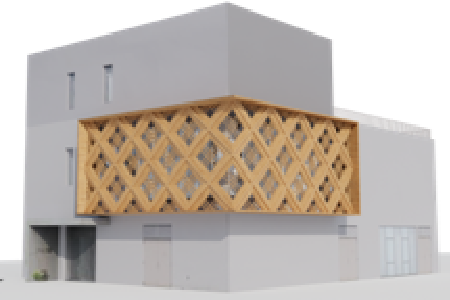
\includegraphics[width=1\linewidth]{Images/CICA3DRender1}} &
                    {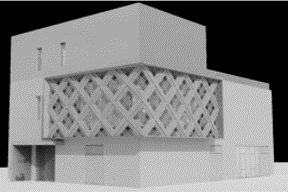
\includegraphics[width=1\linewidth]{Images/CICA3DRender2}} &
                  {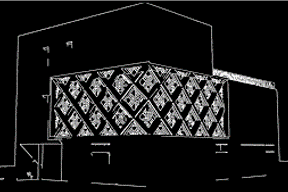
\includegraphics[width=1\linewidth]{Images/CICA3DRender3}} &
                  {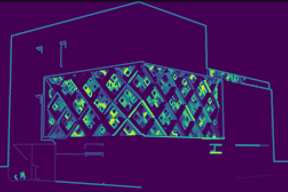
\includegraphics[width=1\linewidth]{Images/CICA3DRender4}} \\
                \midrule
                \text{(b) Historical Analysis} &  &  &
                \\
                {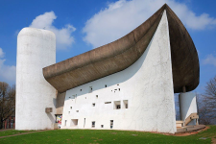
\includegraphics[width=1\linewidth]{Images/CICAHistory1}} &
                    {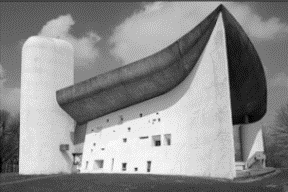
\includegraphics[width=1\linewidth]{Images/CICAHistory2}} &
                  {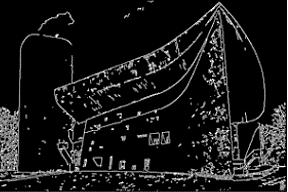
\includegraphics[width=1\linewidth]{Images/CICAHistory3}} &
                  {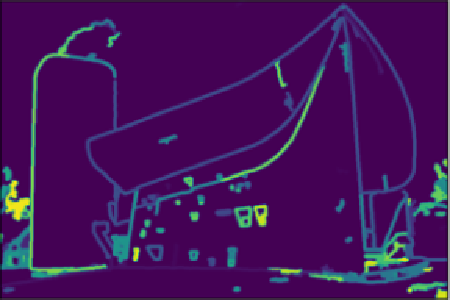
\includegraphics[width=1\linewidth]{Images/CICAHistory4}}\\
                \bottomrule
            \end{tabularx}
        \end{minipage}
    \end{tabular}
    \end{table*}

    %Cica scatter graph for renders
    \begin{table*}[!htb]
    \centering
    \small
    \begin{tabular}{c}
        %Top cell with one figure
        %Scatter graph CICA renders
        \begin{minipage}{\textwidth}
        \centering
        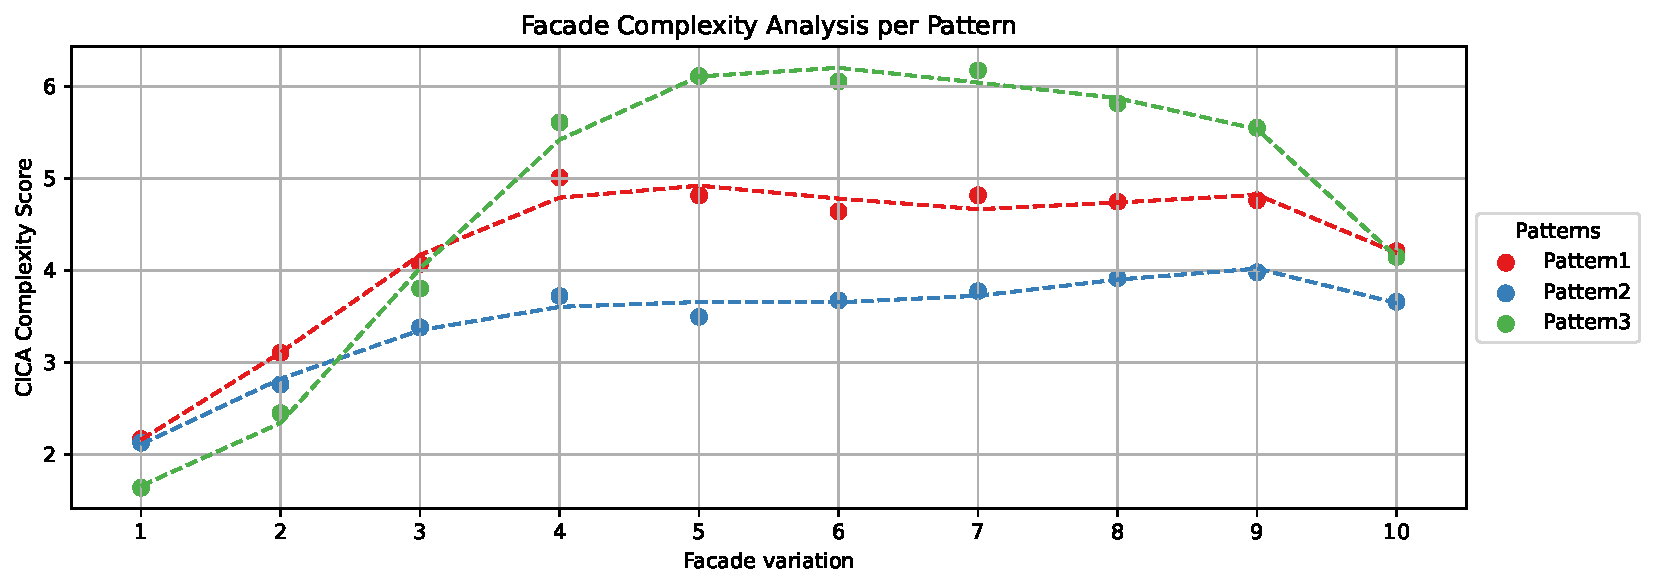
\includegraphics[width= \linewidth]{Graphs/complexitygraphrender}
        \captionof{figure}{Scatter Graph Analysis of 3d modeled Facade Complexity: This graph presents the CICA scores for ten variations of three distinct patterns created in Blender, with a trendline indicating the range of complexity levels among the facade designs, illustrating the nuanced relationship between design intricacy and CICA scores.}
        \label{fig:CICAscatterGraphRender}
        \end{minipage}
    \end{tabular}
    \end{table*}

%!% CICA Metrics and Function
    %PI table, Function1. Table 1x3
    \begin{table*}[!htb]
    \centering
    \small
    \begin{tabular}{c}
        %Top cell with one figure
        %Table: Performance Indicators
        \begin{minipage}{\textwidth}
            \centering
            \captionof{table}{Table of Metrics and Weights for Complexity Scoring: Outlines the key criteria and corresponding weights utilized in the Computational Image Complexity Analysis (CICA) to determine the `Complexity Score' of architectural facades, detailing the systematic approach to quantifying facade intricacy through edge density and contour count metrics.}
            \label{tab:MetricsandWeights}
            \begin{tabularx}{\textwidth}{p{2.5cm} p{1cm} X X p{1cm}}
                \toprule
                \textit{Complexity metric} &
                  \textit{N} &
                  \textit{Metric name/description} &
                  \textit{Quantitative   method} &
                  \textit{Weights} \\ \midrule
                \textbf{Edge Density} &
                  1 &
                  Edge detection using Canny Edge Detection algorithm for highlighting the most relevant features of a building.
                    &
                  Measured by dividing the number of non-zero (edge) pixels in the edges image by the total number of pixels in the image.
                    &
                  8\\
                \textbf{Contour count} &
                  2 &
                  Employs contour approximation algorithm for shape analysis to determine intricacy of edges.
                    &
                  Measure by counting the number of segments in an edge.
                    &
                  2\\ \bottomrule
                   &
                   &
                  \textbf{TOTAL} &
                  &
                  \textbf{10}\\ \bottomrule
            \end{tabularx}
        \end{minipage}
        \\
        \\
        %Middle cell with two nested figures side by side
        %Table function 1 complexity score
        \begin{minipage}{\textwidth}
            \centering
            \captionof{table}{Function 1: Complexity scoring function that integrates various criteria to assess the intricacy of a building facade.}
            \label{tab:ComplexityScoreFunction}
        \begin{tabularx}{\linewidth}{|X|}
            \hline
            \small
            \vspace{-0.1cm}
            \multicolumn{1}{c}{\textbf{\(f_1\): Unified Complexity Scoring Function}}\\
            \textit{Calculate the complexity score for all images in the data pool.}
            \begin{equation}
                f_1(x) = \mathrm{round}\left(\sum_{i=1}^{n} w_i \cdot a_i, 2\right) = \text{complexity\_score}
                \label{eq:F1_ComplexityScoreFunction}
            \end{equation}
            \textit{for the buildings included in the database.}
            \vspace{0.5em}

            \textit{where:}\\
            \(n\): number of performance indicators\\
            \(w_i\): weight of the \(i\)-th element\\
            \(a_i\): normalized score for the \(i\)-th metric (e.g., `Edge Density' and `Contour Count')\\
            \vspace{0.05em}
            \textit{Finally, the "Complexity Score" is assigned to each building for data visualization.}
            \vspace{0.5em}\\
            \hline
        \end{tabularx}
        \end{minipage}
    \end{tabular}
    \end{table*}

    %Table of Cica on historical buildings and renders, Cica evaluation process table. Table 1x3
    \begin{table*}[!htb]
    \centering
    \small
    \begin{tabular}{c}
        %Top cell with one figure
        %Table: CICA Image evaluation process for historical and 3d facades
        \begin{minipage}{\textwidth}
            \centering
            \captionof{table}{CICA Evaluation on Architectural Facades: The table presents a comparative analysis of CICA evaluation applied to 3D-modeled facades (a) and historical buildings (b). The process includes steps from original imagery to image processing (noise reduction, grayscale), edge detection, and contour count analysis, as shown on the flowchart in Figure\ref{fig:CICAImageEvaluationFlowchart}. It highlights  the adaptability of CICA to assess complexity in both historical and contemporary architectural designs.}
            \label{tab:CICAImageEvalProcessOnArchitecturalFacades}
            \begin{tabularx}
            {\textwidth}{X X X X }
                \toprule
                \multicolumn{4}{c}{\textbf{CICA Image Evaluation process on Architectural Facades}} \\
                \toprule
                \multicolumn{1}{c}{\textit{Original Image}} &
                 \multicolumn{1}{c}{\textit{Grayscale, noise reduction}} &
                \multicolumn{1}{c}{\textit{Edge detection Image}} &
                \multicolumn{1}{c}{\textit{Contour count Image}}\\
                \midrule
                \text{(a) 3D-modeled facades} &  &  &
                \\
                {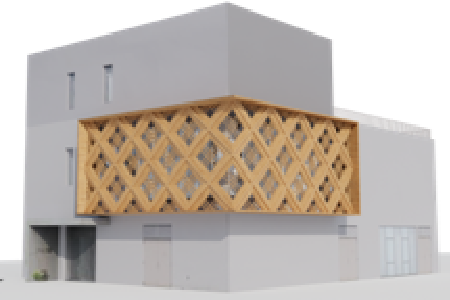
\includegraphics[width=1\linewidth]{Images/CICA3DRender1}} &
                    {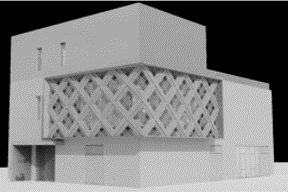
\includegraphics[width=1\linewidth]{Images/CICA3DRender2}} &
                  {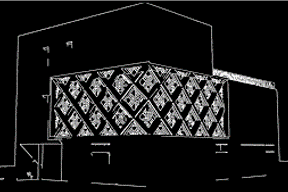
\includegraphics[width=1\linewidth]{Images/CICA3DRender3}} &
                  {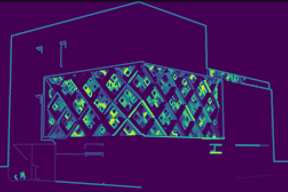
\includegraphics[width=1\linewidth]{Images/CICA3DRender4}} \\
                \midrule
                \text{(b) Historical Analysis} &  &  &
                \\
                {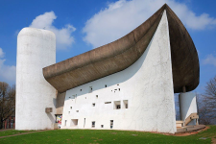
\includegraphics[width=1\linewidth]{Images/CICAHistory1}} &
                    {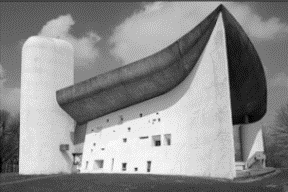
\includegraphics[width=1\linewidth]{Images/CICAHistory2}} &
                  {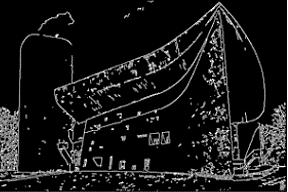
\includegraphics[width=1\linewidth]{Images/CICAHistory3}} &
                  {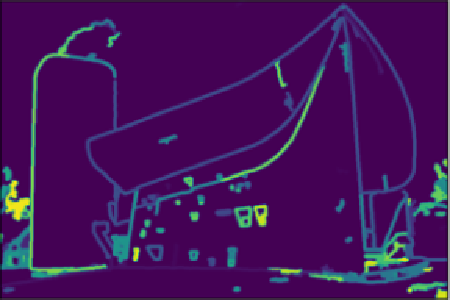
\includegraphics[width=1\linewidth]{Images/CICAHistory4}}\\
                \bottomrule
            \end{tabularx}
        \end{minipage}
        \\
        \\
        %Bottom cell
        %Scatter graph CICA renders
        \begin{minipage}{\textwidth}
        \centering
        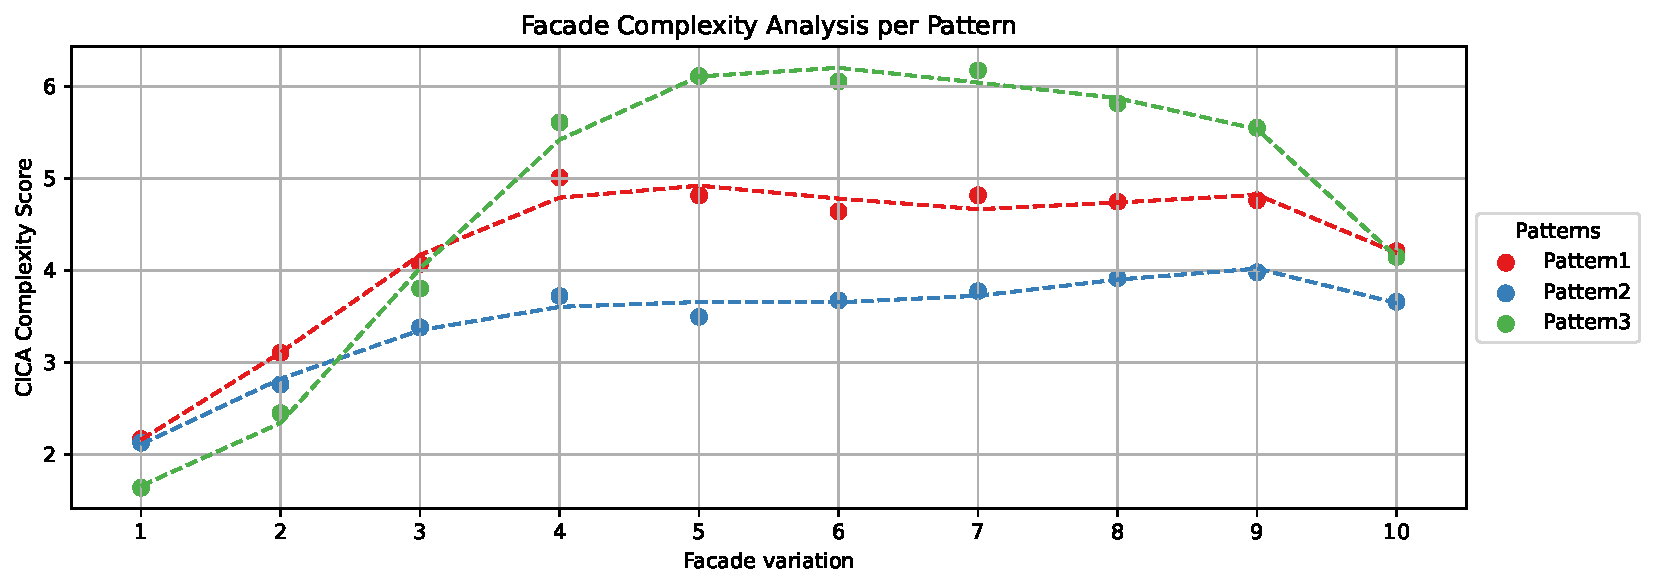
\includegraphics[width= \linewidth]{Graphs/complexitygraphrender}
        \captionof{figure}{Scatter Graph Analysis of 3d modeled Facade Complexity: This graph presents the CICA scores for ten variations of three distinct patterns created in Blender, with a trendline indicating the range of complexity levels among the facade designs, illustrating the nuanced relationship between design intricacy and CICA scores.}
        \label{fig:CICAscatterGraphRender}
        \end{minipage}
    \end{tabular}
    \end{table*}


%!% CICA tables and function
    %Table of Cica on historical buildings and renders, PI table, Function1. Table 1x3
    \begin{table*}[!htb]
    \centering
    \small
    \begin{tabular}{c}
        %Top cell with one figure
        %Table: Performance Indicators
        \begin{minipage}{\textwidth}
            \centering
            \captionof{table}{Table of Metrics and Weights for Complexity Scoring: Outlines the key criteria and corresponding weights utilized in the Computational Image Complexity Analysis (CICA) to determine the `Complexity Score' of architectural facades, detailing the systematic approach to quantifying facade intricacy through edge density and contour count metrics.}
            \label{tab:MetricsandWeights}
            \begin{tabularx}{\textwidth}{p{2.5cm} p{1cm} X X p{1cm}}
                \toprule
                \textit{Complexity metric} &
                  \textit{N} &
                  \textit{Metric name/description} &
                  \textit{Quantitative   method} &
                  \textit{Weights} \\ \midrule
                \textbf{Edge Density} &
                  1 &
                  Edge detection using Canny Edge Detection algorithm for highlighting the most relevant features of a building.
                    &
                  Measured by dividing the number of non-zero (edge) pixels in the edges image by the total number of pixels in the image.
                    &
                  8\\
                \textbf{Contour count} &
                  2 &
                  Employs contour approximation algorithm for shape analysis to determine intricacy of edges.
                    &
                  Measure by counting the number of segments in an edge.
                    &
                  2\\ \bottomrule
                   &
                   &
                  \textbf{TOTAL} &
                  &
                  \textbf{10}\\ \bottomrule
            \end{tabularx}
        \end{minipage}
        \\
        \\
        %Middle cell with two nested figures side by side
        %Table: CICA Image evaluation process for historical and 3d facades
        \begin{minipage}{\textwidth}
            \centering
            \captionof{table}{CICA Evaluation on Architectural Facades: The table presents a comparative analysis of CICA evaluation applied to 3D-modeled facades (a) and historical buildings (b). The process includes steps from original imagery to image processing (noise reduction, grayscale), edge detection, and contour count analysis, as shown on the flowchart in Figure\ref{fig:CICAImageEvaluationFlowchart}. It highlights  the adaptability of CICA to assess complexity in both historical and contemporary architectural designs.}
            \label{tab:CICAImageEvalProcessOnArchitecturalFacades}
            \begin{tabularx}
            {\textwidth}{X X X X }
                \toprule
                \multicolumn{4}{c}{\textbf{CICA Image Evaluation process on Architectural Facades}} \\
                \toprule
                \multicolumn{1}{c}{\textit{Original Image}} &
                 \multicolumn{1}{c}{\textit{Grayscale, noise reduction}} &
                \multicolumn{1}{c}{\textit{Edge detection Image}} &
                \multicolumn{1}{c}{\textit{Contour count Image}}\\
                \midrule
                \text{(a) 3D-modeled facades} &  &  &
                \\
                {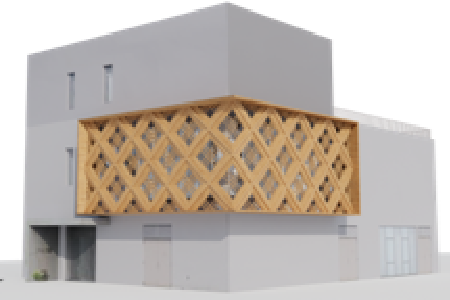
\includegraphics[width=1\linewidth]{Images/CICA3DRender1}} &
                    {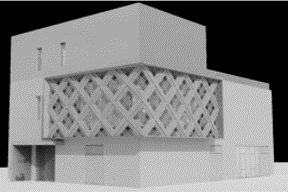
\includegraphics[width=1\linewidth]{Images/CICA3DRender2}} &
                  {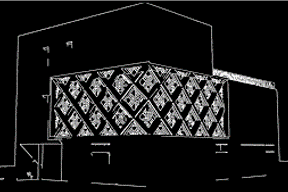
\includegraphics[width=1\linewidth]{Images/CICA3DRender3}} &
                  {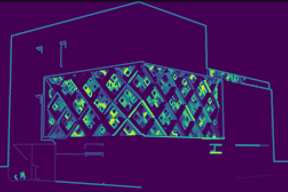
\includegraphics[width=1\linewidth]{Images/CICA3DRender4}} \\
                \midrule
                \text{(b) Historical Analysis} &  &  &
                \\
                {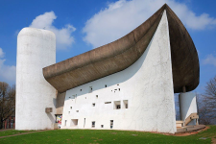
\includegraphics[width=1\linewidth]{Images/CICAHistory1}} &
                    {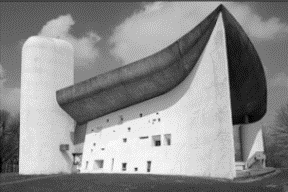
\includegraphics[width=1\linewidth]{Images/CICAHistory2}} &
                  {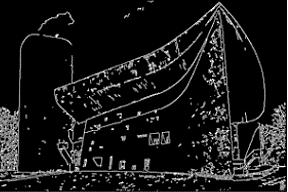
\includegraphics[width=1\linewidth]{Images/CICAHistory3}} &
                  {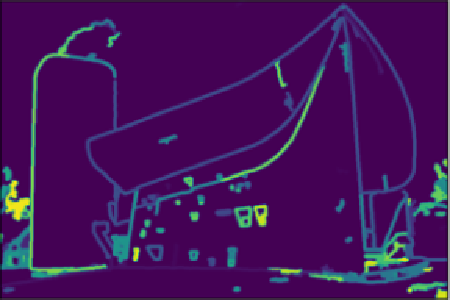
\includegraphics[width=1\linewidth]{Images/CICAHistory4}}\\
                \bottomrule
            \end{tabularx}
        \end{minipage}
        \\
        \\
        %Bottom cell
        %Table function 1 complexity score
        \begin{minipage}{\textwidth}
            \centering
            \captionof{table}{Function 1: Complexity scoring function that integrates various criteria to assess the intricacy of a building facade.}
            \label{tab:ComplexityScoreFunction}
        \begin{tabularx}{\linewidth}{|X|}
            \hline
            \small
            \vspace{-0.1cm}
            \multicolumn{1}{c}{\textbf{\(f_1\): Unified Complexity Scoring Function}}\\
            \textit{Calculate the complexity score for all images in the data pool.}
            \begin{equation}
                f_1(x) = \mathrm{round}\left(\sum_{i=1}^{n} w_i \cdot a_i, 2\right) = \text{complexity\_score}
                \label{eq:F1_ComplexityScoreFunction}
            \end{equation}
            \textit{for the buildings included in the database.}
            \vspace{0.5em}

            \textit{where:}\\
            \(n\): number of performance indicators\\
            \(w_i\): weight of the \(i\)-th element\\
            \(a_i\): normalized score for the \(i\)-th metric (e.g., `Edge Density' and `Contour Count')\\
            \vspace{0.05em}
            \textit{Finally, the "Complexity Score" is assigned to each building for data visualization.}
            \vspace{0.5em}\\
            \hline
        \end{tabularx}
        \end{minipage}
    \end{tabular}
    \end{table*}

%! Function for complexity score
    %%Table function 1 complexity score
    \begin{table*}[htb]
        \caption{Function 1: Complexity scoring function that integrates various criteria to assess the intricacy of a building facade.}
        \label{tab:ComplexityScoreFunction}
        \begin{tabularx}{\linewidth}{|X|}
            \hline
            \small
            \vspace{-0.1cm}
            \multicolumn{1}{c}{\textbf{\(f_1\): Unified Complexity Scoring Function}}\\
            \textit{Calculate the complexity score for all images in the data pool.}
            \begin{equation}
                f_1(x) = \mathrm{round}\left(\sum_{i=1}^{n} w_i \cdot a_i, 2\right) = \text{complexity\_score}
                \label{eq:F1_ComplexityScoreFunction}
            \end{equation}
            \textit{for the buildings included in the database.}
            \vspace{0.5em}

            \textit{where:}\\
            \(n\): number of performance indicators\\
            \(w_i\): weight of the \(i\)-th element\\
            \(a_i\): normalized score for the \(i\)-th metric (e.g., `Edge Density' and `Contour Count')\\
            \vspace{0.05em}
            \textit{Finally, the "Complexity Score" is assigned to each building for data visualization.}
            \vspace{0.5em}\\
            \hline
        \end{tabularx}
    \end{table*}

%!%Figures and table CICA
%Flowchart CICA, Table of Cica on historical buildings and renders, PI table. Table 1x3
\begin{table*}[!htb]
\centering
\small
\begin{tabular}{c}
    %Top cell with one figure
    %Figure Computational Image Compexity Analysis (CICA) System flowchart
    \begin{minipage}{\textwidth}
        \centering
        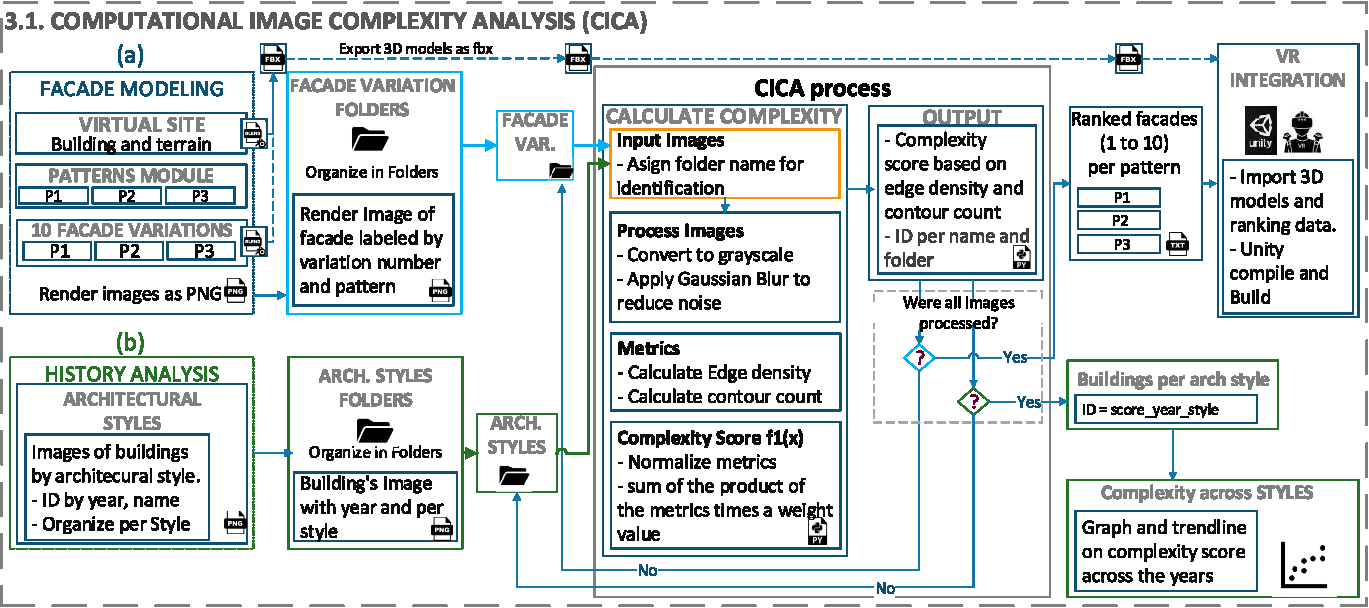
\includegraphics[width= \linewidth]{Images/CICAFlowchart}
        \captionof{figure}{Flowchart illustrating the applications of Computational Image Complexity Analysis system (CICA)(detailed in Section\ref{subsec:Computational Image Complexity analysis}), including its role in analyzing complexity scores for historical architectural styles (b) and 3D-modeled facades (a) designed with various degrees of complexity(presented in Section\ref{subsubsec:CICAforFacades}).}
        \label{fig:CICAImageEvaluationFlowchart}
    \end{minipage}
    \\
    \\
    %Middle cell with two nested figures side by side
    %Table: Performance Indicators
    \begin{minipage}{\textwidth}
        \centering
        \captionof{table}{Table of Metrics and Weights for Complexity Scoring: Outlines the key criteria and corresponding weights utilized in the Computational Image Complexity Analysis (CICA) to determine the `Complexity Score' of architectural facades, detailing the systematic approach to quantifying facade intricacy through edge density and contour count metrics.}
        \label{tab:MetricsandWeights}
        \begin{tabularx}{\textwidth}{p{2.5cm} p{1cm} X X p{1cm}}
            \toprule
            \textit{Complexity metric} &
              \textit{N} &
              \textit{Metric name/description} &
              \textit{Quantitative   method} &
              \textit{Weights} \\ \midrule
            \textbf{Edge Density} &
              1 &
              Edge detection using Canny Edge Detection algorithm for highlighting the most relevant features of a building.
                &
              Measured by dividing the number of non-zero (edge) pixels in the edges image by the total number of pixels in the image.
                &
              8\\
            \textbf{Contour count} &
              2 &
              Employs contour approximation algorithm for shape analysis to determine intricacy of edges.
                &
              Measure by counting the number of segments in an edge.
                &
              2\\ \bottomrule
               &
               &
              \textbf{TOTAL} &
              &
              \textbf{10}\\ \bottomrule
        \end{tabularx}
    \end{minipage}
    \\
    \\
    %Bottom cell
    %Table: CICA Image evaluation process for historical and 3d facades
    \begin{minipage}{\textwidth}
        \centering
        \captionof{table}{CICA Evaluation on Architectural Facades: The table presents a comparative analysis of CICA evaluation applied to 3D-modeled facades (a) and historical buildings (b). The process includes steps from original imagery to image processing (noise reduction, grayscale), edge detection, and contour count analysis, as shown on the flowchart in Figure\ref{fig:CICAImageEvaluationFlowchart}. It highlights  the adaptability of CICA to assess complexity in both historical and contemporary architectural designs.}
        \label{tab:CICAImageEvalProcessOnArchitecturalFacades}
        \begin{tabularx}
        {\textwidth}{X X X X }
            \toprule
            \multicolumn{4}{c}{\textbf{CICA Image Evaluation process on Architectural Facades}} \\
            \toprule
            \multicolumn{1}{c}{\textit{Original Image}} &
             \multicolumn{1}{c}{\textit{Grayscale, noise reduction}} &
            \multicolumn{1}{c}{\textit{Edge detection Image}} &
            \multicolumn{1}{c}{\textit{Contour count Image}}\\
            \midrule
            \text{(a) 3D-modeled facades} &  &  &
            \\
            {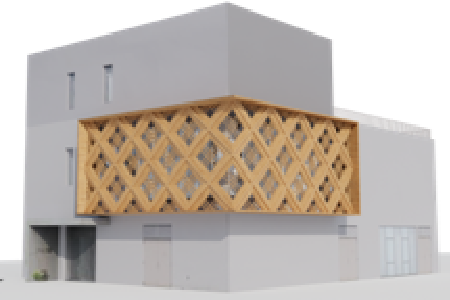
\includegraphics[width=1\linewidth]{Images/CICA3DRender1}} &
                {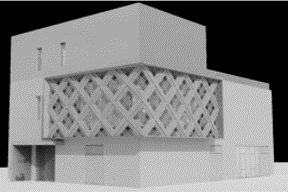
\includegraphics[width=1\linewidth]{Images/CICA3DRender2}} &
              {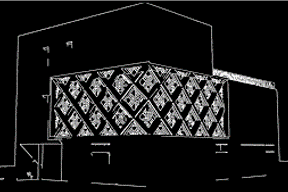
\includegraphics[width=1\linewidth]{Images/CICA3DRender3}} &
              {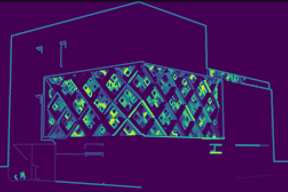
\includegraphics[width=1\linewidth]{Images/CICA3DRender4}} \\
            \midrule
            \text{(b) Historical Analysis} &  &  &
            \\
            {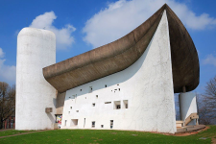
\includegraphics[width=1\linewidth]{Images/CICAHistory1}} &
                {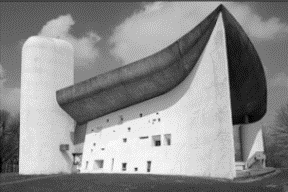
\includegraphics[width=1\linewidth]{Images/CICAHistory2}} &
              {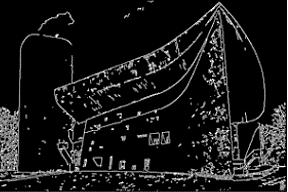
\includegraphics[width=1\linewidth]{Images/CICAHistory3}} &
              {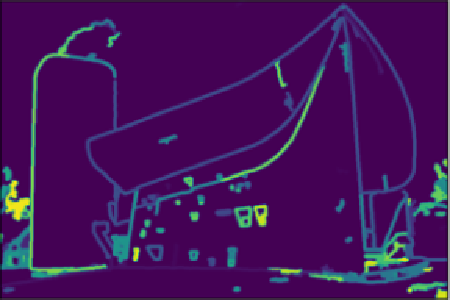
\includegraphics[width=1\linewidth]{Images/CICAHistory4}}\\
            \bottomrule
        \end{tabularx}
    \end{minipage}
\end{tabular}
\end{table*}


%! CiCA algorithm table
%%Table: CICA Image Process for historical and 3d modeled facades
\begin{table*}[htb]
    \centering
    \small
    \caption{CICA Evaluation on Architectural Facades: The table presents a comparative analysis of CICA evaluation applied to historical buildings (top row) and 3D-modeled facades (bottom row). The process includes steps from original imagery to image processing, edge detection, and contour count analysis, highlighting  the adaptability of CICA to assess complexity in both historical and contemporary architectural designs.}
    \label{tab:CICAPlotMaster}
    \begin{tabularx}
    {\textwidth}{X X X X }
        \toprule
        \multicolumn{4}{c}{\textbf{CICA Image Evaluation process}} \\
        \midrule
        \textit{Original Image} &
          \textit{Grayscale, noise reduction} &
          \textit{Edge detection Image} &
          \textit{Contour count Image}\\
        \midrule
        \text{(a) 3D-modeled facades} &  &  &
        \\
        {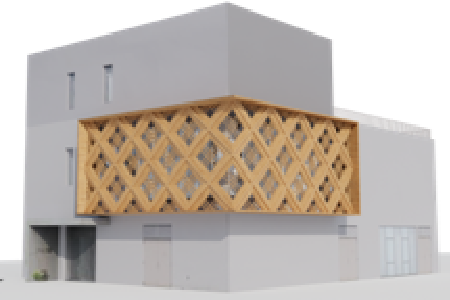
\includegraphics[width=1\linewidth]{Images/CICA3DRender1}} &
            {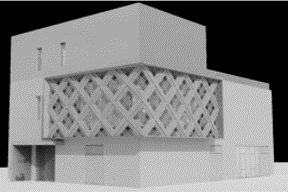
\includegraphics[width=1\linewidth]{Images/CICA3DRender2}} &
          {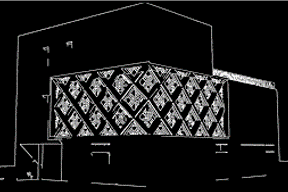
\includegraphics[width=1\linewidth]{Images/CICA3DRender3}} &
          {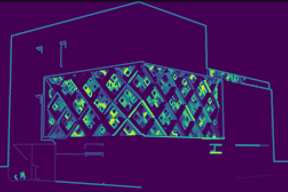
\includegraphics[width=1\linewidth]{Images/CICA3DRender4}} \\
        \midrule
        \text{(b) Historical Analysis} &  &  &
        \\
        {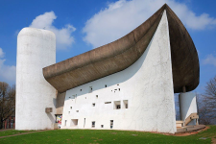
\includegraphics[width=1\linewidth]{Images/CICAHistory1}} &
            {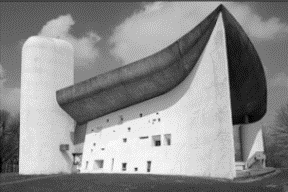
\includegraphics[width=1\linewidth]{Images/CICAHistory2}} &
          {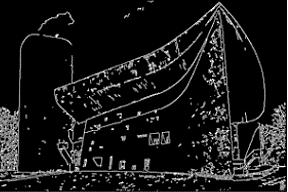
\includegraphics[width=1\linewidth]{Images/CICAHistory3}} &
          {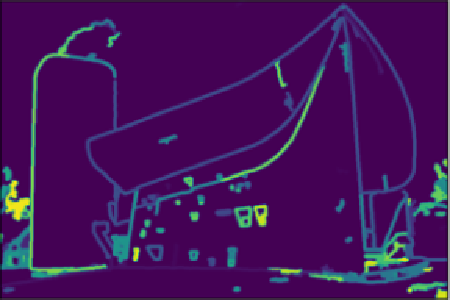
\includegraphics[width=1\linewidth]{Images/CICAHistory4}}\\
        \bottomrule
    \end{tabularx}
\end{table*}

%!Results pages

%Table 1x2
% Accuracy graphs of complexity ranking per pattern
% Survey question graph
\begin{table*}[htb]
    \centering
    \small
    \begin{tabular}{c}
        %Top cell with one figure
        %Accuracy graphs of complexity ranking per pattern as a single image
        \begin{minipage}{\textwidth}
            \centering
            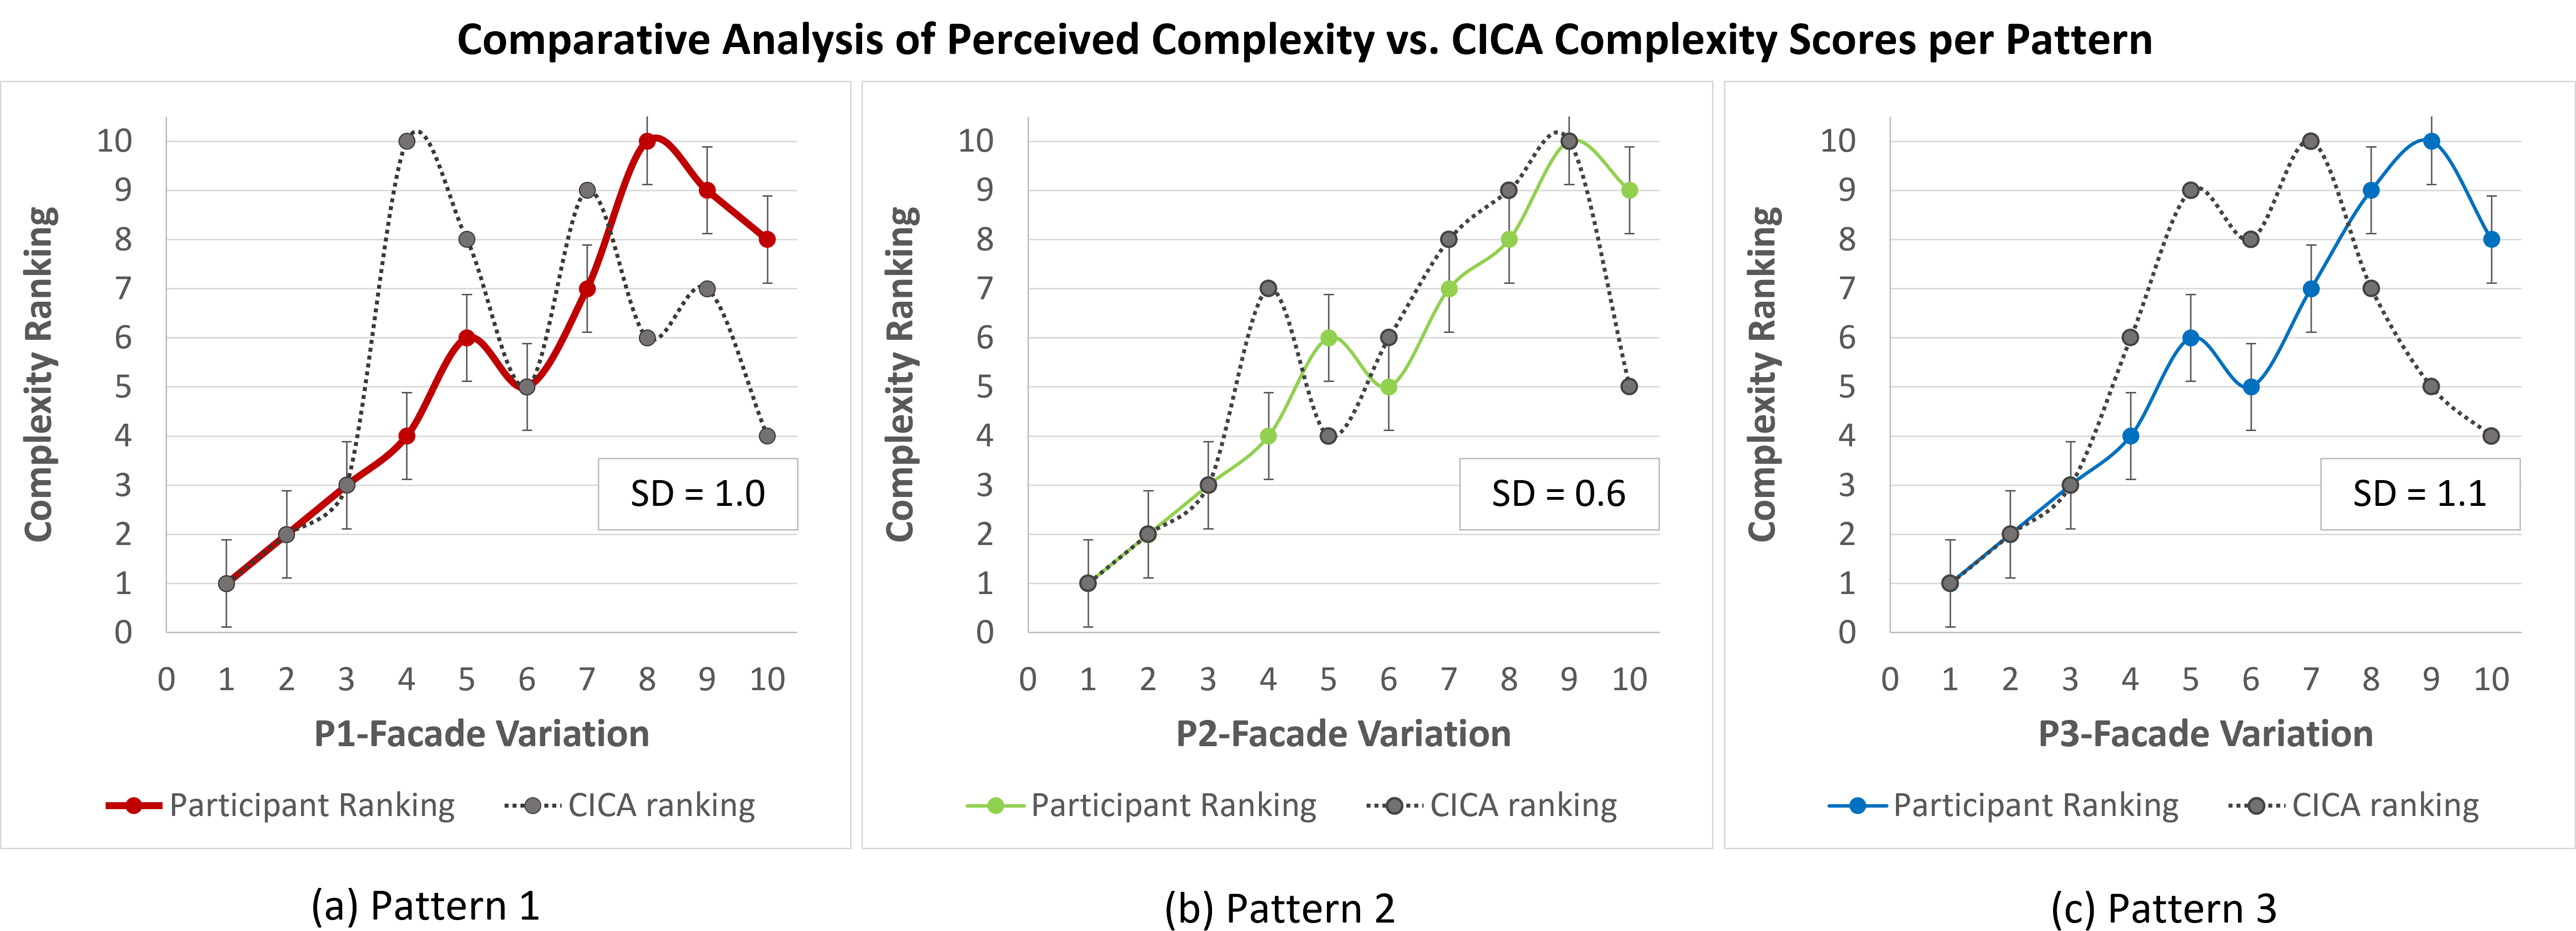
\includegraphics[width=\linewidth]{Images/AccuracyPatternMaster}
            \captionof{figure}{Comparative Analysis of Perceived Complexity vs. CICA Complexity Scores per Pattern: This line graph series illustrates the difference between participants' perceived complexity rankings and the objective CICA scores for facade variations within three distinct patterns. The graphs are presented from left to right: Pattern 1 (a), Pattern 2 (b), and Pattern 3 (c). The ranking line shows the complexity assessment from least (1) to most complex (10),highlighting the contrast between human perception and computational analysis in evaluating architectural complexity.}
            \label{fig:AccuracyPatternMaster}
        \end{minipage}
        \\
        %Bottom cell with two nested figures side by side
        %Survey question graphs
        \begin{minipage}{\textwidth}
            \centering
            % Left figure
            % Survey question 6 to 10
            \begin{minipage}{0.49\textwidth}
                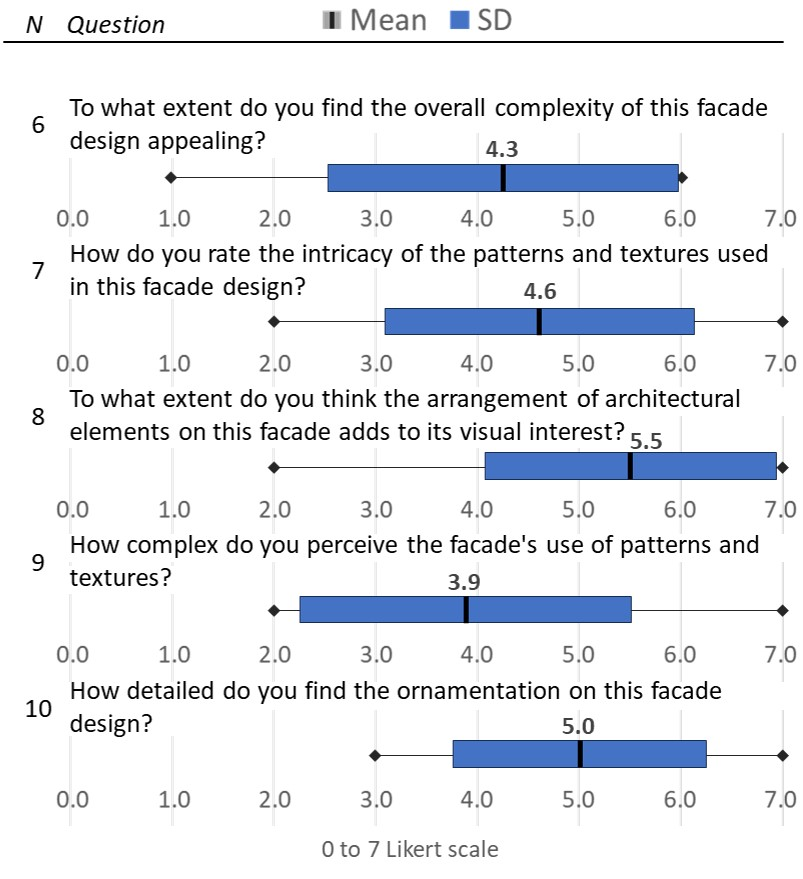
\includegraphics[width=\linewidth]{Images/SurveyPart1Complexity}
                \captionof{figure}{Questions 6 to 10 of the Complexity perception section from the Post-Experiment Survey. \- (n = 10), 1 - strongly disagree, 7 - strongly agree}
                \label{fig:SurveyQuestions6-10}
            \end{minipage}
            \hfill % Spacing between the figures
            % Right figure
            % Survey question 11 to 15
            \begin{minipage}{0.49\textwidth}
                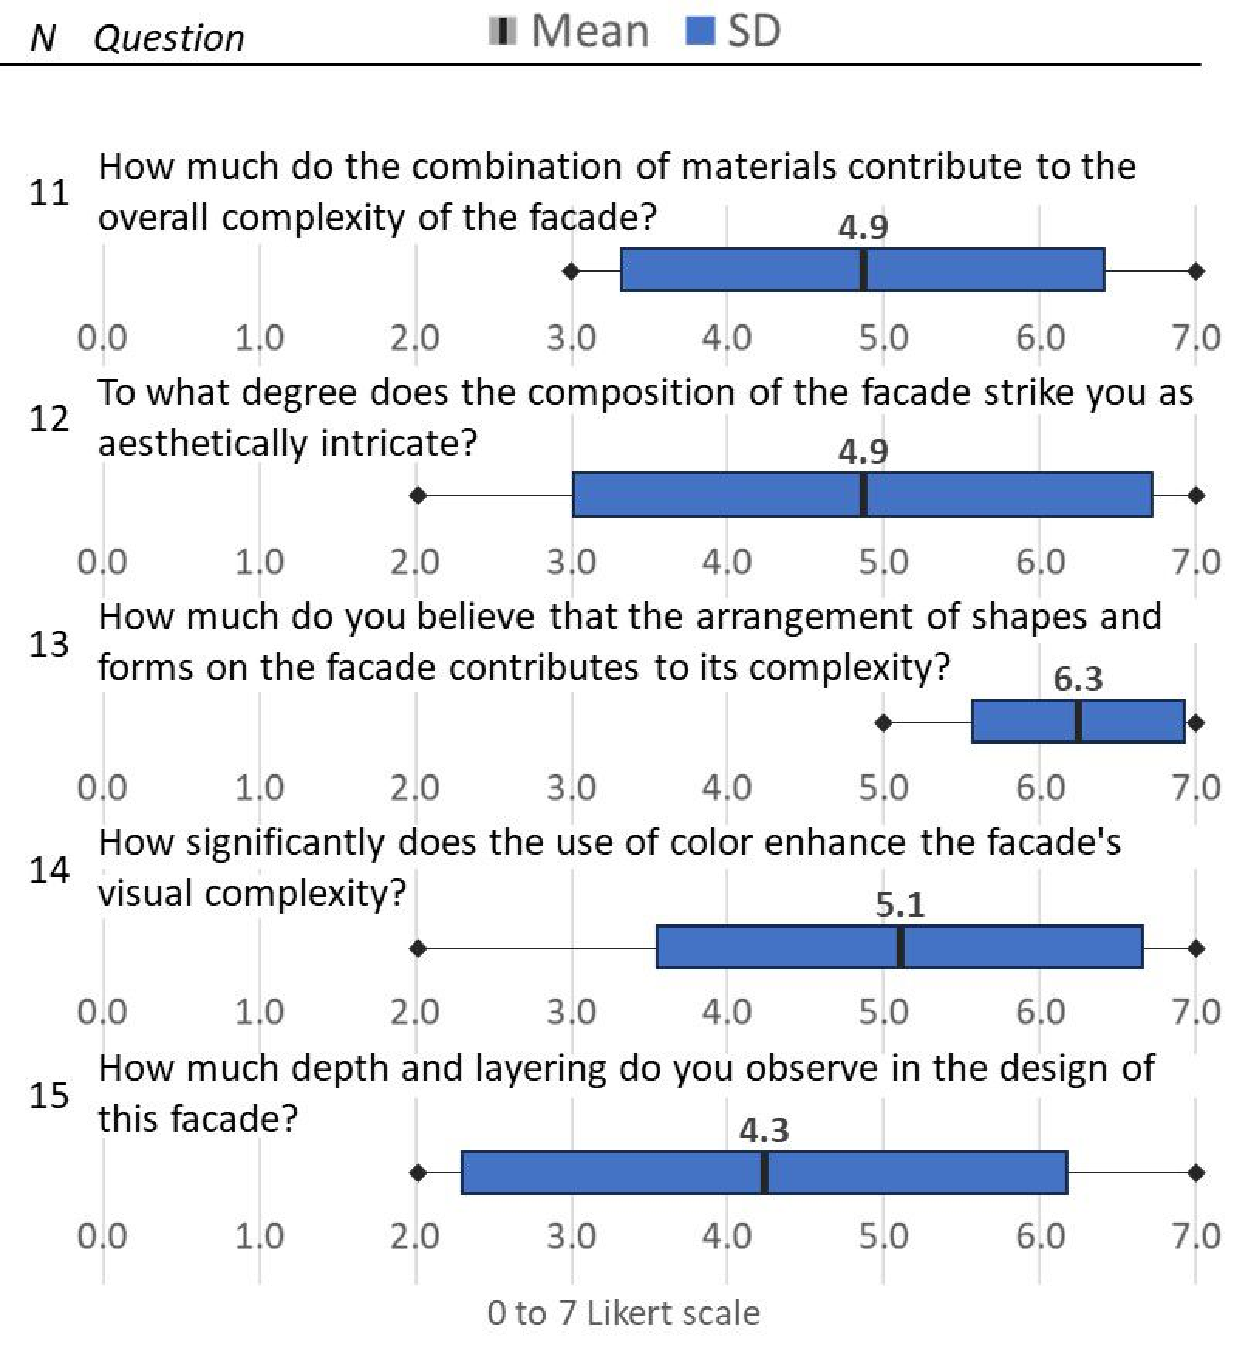
\includegraphics[width=\linewidth]{Images/SurveyPart2Complexity}
                \captionof{figure}{Questions 11 to 15 of the Complexity perception section from the Post-Experiment Survey. \- (n = 10), 1 - strongly disagree, 7 - strongly agree}
                \label{fig:SurveyQuestions11-15}
            \end{minipage}
        \end{minipage}
    \end{tabular}
\end{table*}

%Table 3x2
%Participant background chart, years of experience, Bar Chart of Chosen facade variation, Probability Chart and Complexity level per Pattern
\begin{table*}[htb]
    \centering
    \small
    \begin{tabular}{c}
        %Top cell with two nested figures side by side
        %Participants background and Years of experience
        \begin{minipage}{\textwidth}
            \centering
            % Left figure
            %Participants background
            \begin{minipage}{0.49\textwidth}
                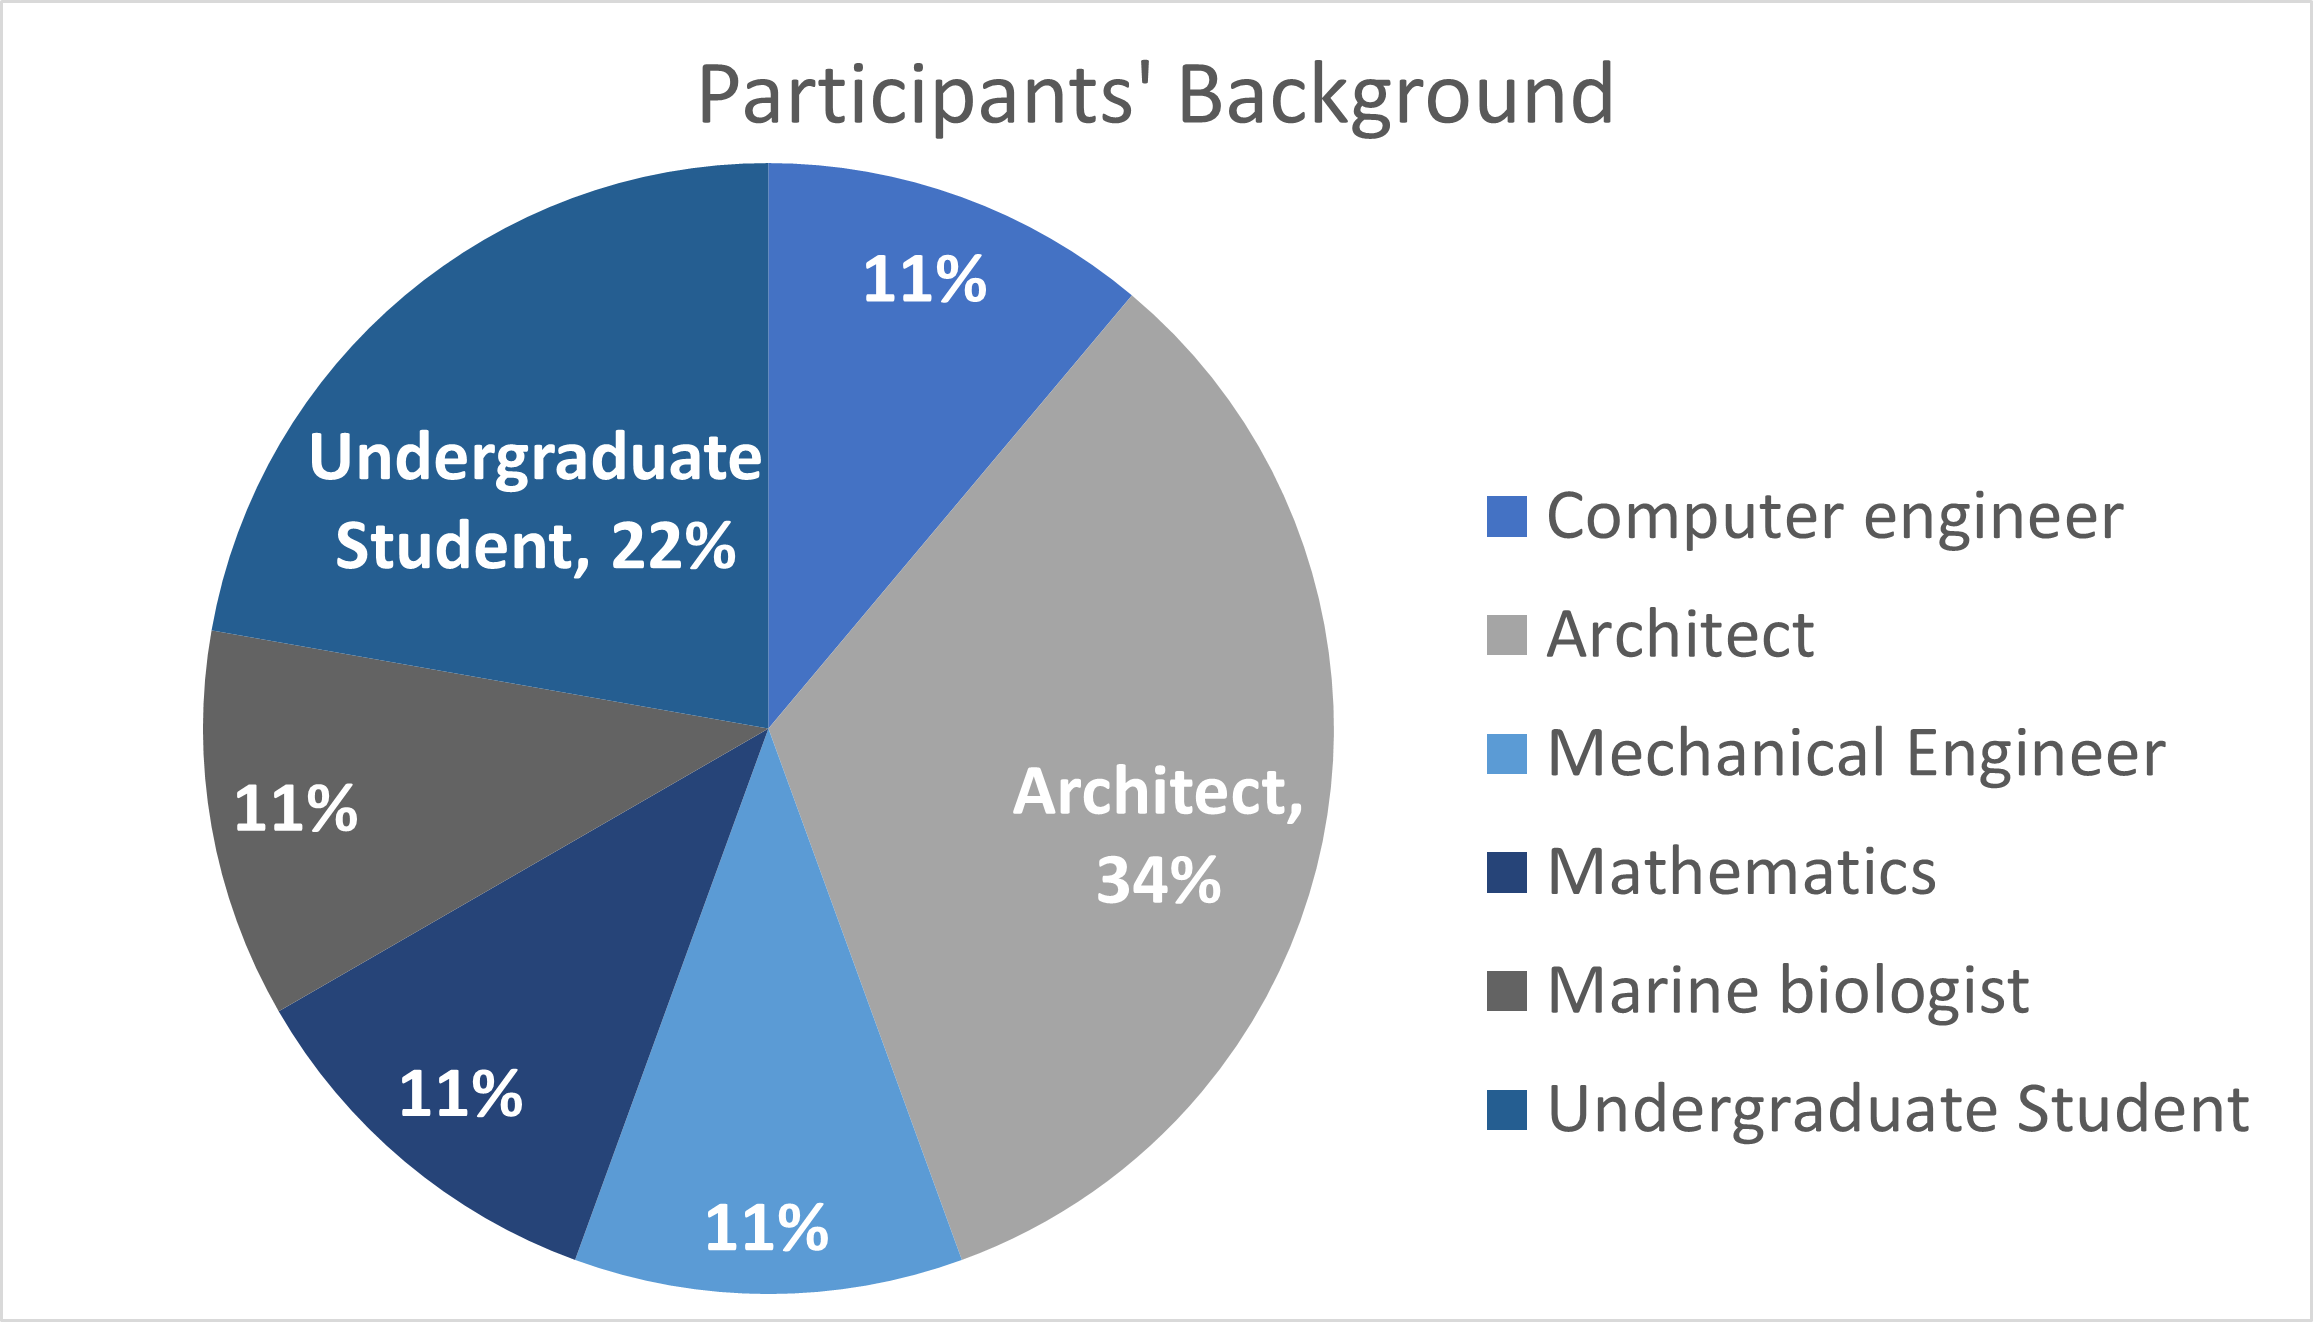
\includegraphics[width=\linewidth, trim=0 60 0 0]{Images/SurveyBackground}
                \captionof{figure}{This chart shows the professional backgrounds of participants involved in the facade design complexity analysis experiment.}
                \label{fig:SurveyBackgroundChart}
            \end{minipage}
            \hfill % Spacing between the figures
            % Right figure
            \begin{minipage}{0.49\textwidth}
                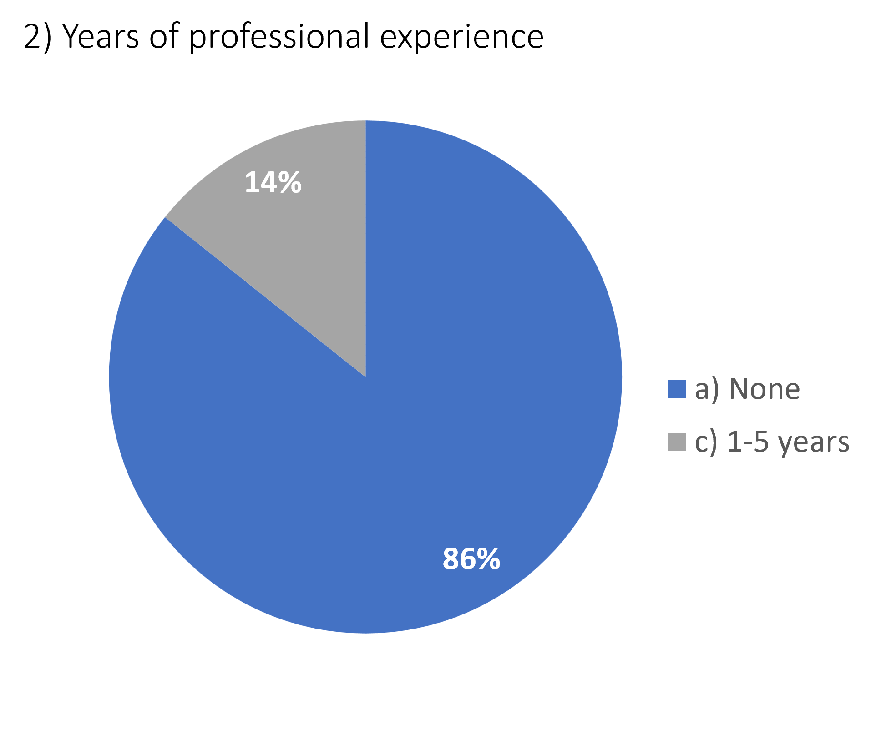
\includegraphics[width=\linewidth, trim=0 60 0 0]{Images/SurveyExperience}
                \captionof{figure}{This chart displays the experience levels in facade design of participants for the study complexity analysis in building design.}
                \label{fig:SurveyYearsExperienceChart}
            \end{minipage}
        \end{minipage}
        \\
        %Middle cell with one figure
        %Facade chosen and CICA score chart per participant
        \begin{minipage}{\textwidth}
            \centering
            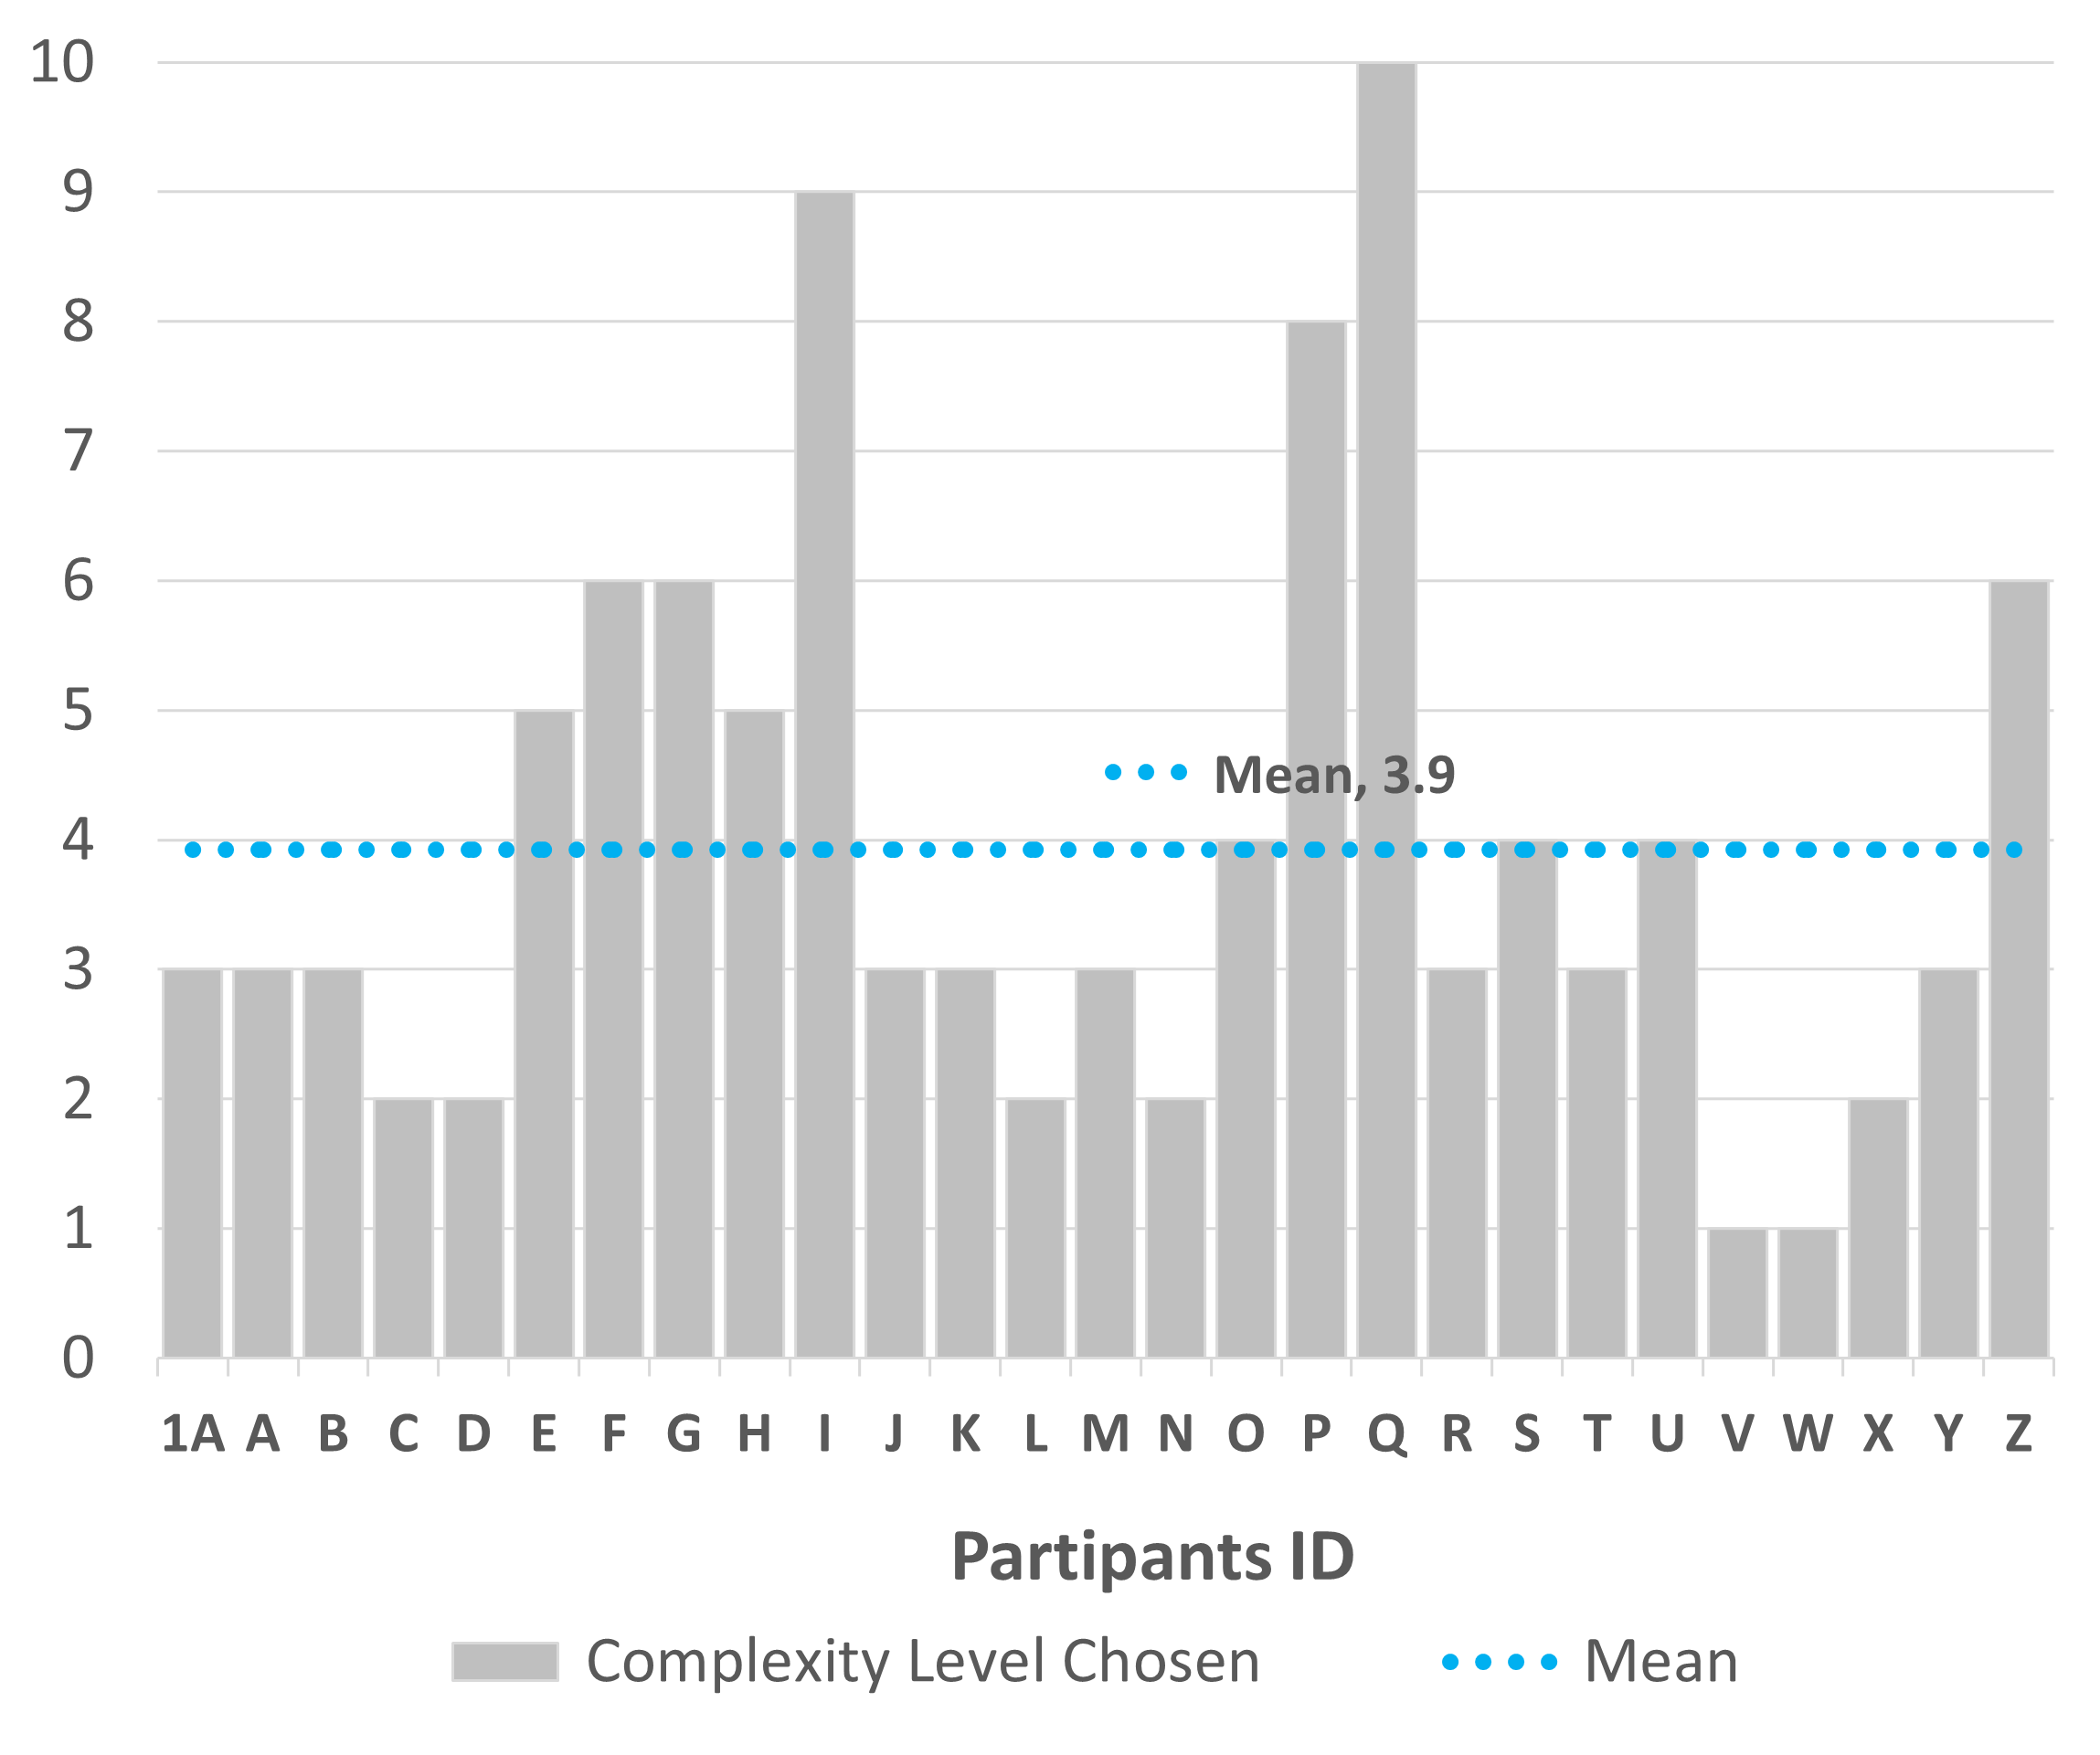
\includegraphics[width=\linewidth]{Images/ComplexityLevelChosenChart}
            \captionof{figure}{Facade Variation Selections and CICA Scores During VR Stage: This chart shows participants' chosen facade variations (bars, height = ID number 1-10) and their CICA complexity scores (line, points = score 0-10) during the VR stage of the experiment. The solid line represents individual CICA scores, while the dotted line indicates the mean average. This visualization highlights the relationship between participant selections and complexity assessment in the immersive VR environmentChart displaying participants' preferred complexity levels among the ten options during the VR simulation stage of the experiment for all three patterns.(CICA Score: Mean = 3.82; SD = 1.1)}
            \label{fig:ComplexityLevelChosenChart}
        \end{minipage}
        \\
        %Bottom cell with two nested figures side by side
        %Probability Chart and Complexity level per Pattern
        \begin{minipage}{\textwidth}
            \centering
            % Left figure
            % Probability Chart
            \begin{minipage}{0.49\textwidth}
                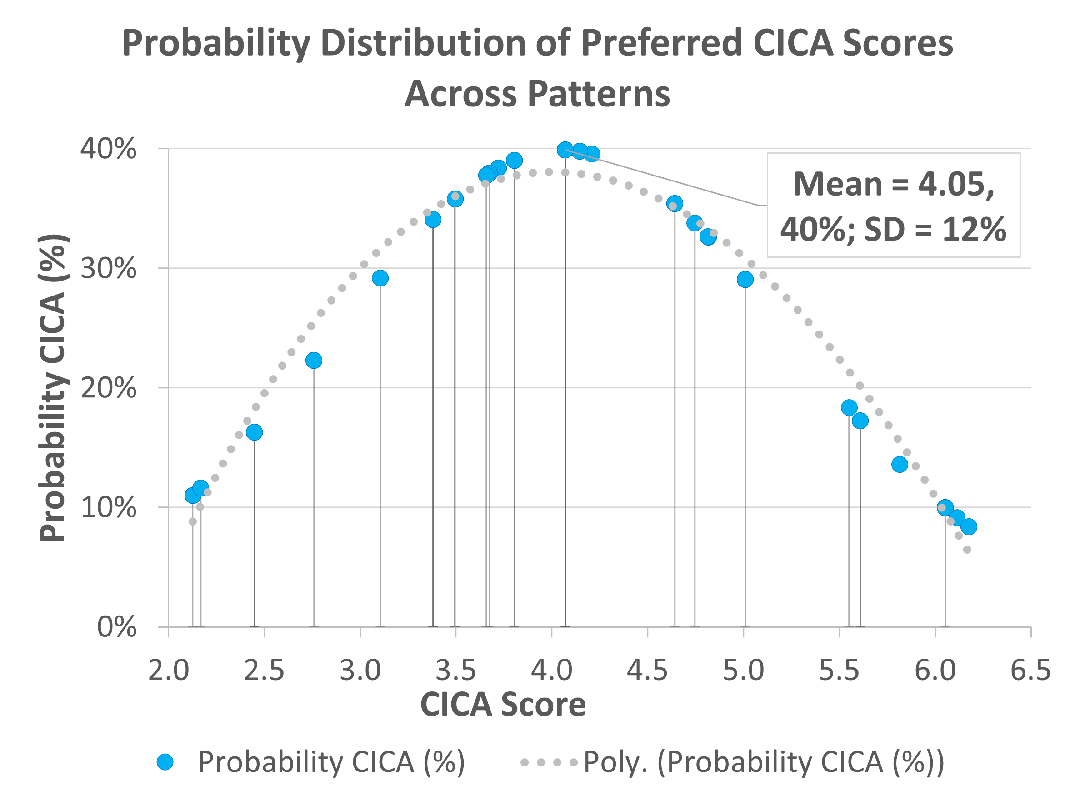
\includegraphics[width=\linewidth]{Images/ProbabilityPreferredComplexitylevel}
                \captionof{figure}{Scatter graph illustrating the probability distribution of preferred CICA score for facade design across all three patterns, derived from data collected during the VR stage of the experiment.(Probability CICA score: \(Mean = 3.82, 40\%\ ; SD = 13\%\))}
                \label{fig:ProbabilityComplexitylevelChart}
            \end{minipage}
            \hfill % Spacing between the figures
            % Right figure
            % Complexity level per Pattern
            \begin{minipage}{0.49\textwidth}
                \includegraphics[width=\linewidth]{Images/PreferredComplexityLevelPerPattern}
                \captionof{figure}{Average CICA score of preferred facade variation per pattern chosen by participants during the VR stage of the experiment. (Facade variation: \(Mean = 3.9\). CICA score: \(Mean = 3.82; SD = 1.1\)).}
                \label{fig:ComplexityLevelPerPattern}
            \end{minipage}
        \end{minipage}
    \end{tabular}
\end{table*}


%! Timeline table 3x1
%%Table function 1 complexity score
\begin{table*}[htb]
    \centering
    \small
    \begin{tabular}{c}
        %Top cell with one figure
        %Figure early timeline
        \begin{minipage}{\textwidth}
            \centering
            \includegraphics[width= \linewidth]{Images/OldTimeline}
                    \captionof{figure}{Early timeline. Sequential representation of architectural styles illustrating the shift between complexity and simplicity. From left to right: Romanesque[a] with its solid and massive structure; Gothic[b] featuring verticality and lightness; Classicism[c] characterized by geometrical clarity and order; Baroque[d] with dynamic shapes and rich decorations; followed by the restrained and symmetrical formality of Neo-classicism[e]. (\textit{Images edited from source})}
                    \label{fig:Oldtimeline}
        \end{minipage}
        \\
        %Middle cell
        %Middle timeline
        \begin{minipage}{\textwidth}
            \centering
            \includegraphics[width= \linewidth]{Images/MiddleTimeline}
                    \captionof{figure}{Transitional timeline. Sequential representation of architectural styles illustrating the shift between complexity and simplicity. From left to right: Art Nouveau[a] with its fluid lines and natural forms; Art Deco[b], marked by bold geometry and opulence; Modernism's[c] pursuit of stripped-back functionality; culminating in Postmodernism's[d] revival of historical styles and complexity (\textit{Images edited from source})}
                    \label{fig:Middletimeline}
        \end{minipage}
        \\
        %bottom Cell
        %Contemporary timeline
        \begin{minipage}{\textwidth}
            \centering
            \includegraphics[width= \linewidth]{Images/contemporaryTimeline}
                    \captionof{figure}{Contemporary timeline. Sequential representation of architectural styles illustrating the shift between complexity and simplicity. Era of exploration and innovation. From left to right: Deconstructivism[a], characterized by fragmentation and non-linear design; Neofuturism[b], capturing movement and technology-infused aesthetics; High-tech modernism[c], focusing on visible structural elements and technological expression; Parametricism[d], with its algorithm-based complex forms; and Pragmatic utopianism[e], blending idealistic designs with practical applications (\textit{Images edited from source})}
                    \label{fig:contemporarytimeline}
        \end{minipage}
    \end{tabular}
\end{table*}


%! Function for complexity score
%%Table function 1 complexity score
\begin{table*}[htb]
\centering
\caption{Function 1: Complexity scoring function that integrates various criteria to assess intricacy of a building facade.}
\label{tab:ComplexityScoreFunction_table}
    \begin{tabular}{|c c|}%{|c|c|}
    \hline
    % First Cell (Top-Left)
    % f1: Valid Position finder function
        \begin{minipage}{.45\linewidth}
            \centering
            \small
            \begin{tabular}{p{8cm}}
                \\
                \textbf{\(f_1\), Unified `Complexity Scoring' function 1}\\
                    \textit{Calculate the complexity score for all the images on the data pool}
                    \\
                    \begin{equation}
                        f_1(x) = \left[ \mathrm{round}\left(\sum_{i=1}^{n} w_i \cdot a_i, 2\right) \right] = complexity\_score
                    \label{eq:F1_ComplexityScoreFunction}
                    \end{equation}
                    \\
                    \textit{ for the Buildings included in the database.}\\
                \\
            \end{tabular}
        \end{minipage}
        &
        % Second Cell (Top-Right)
        % continuation f1
        \begin{minipage}{.45\linewidth}
            \centering
            \small
            \begin{tabular}{p{8cm}}
                \\\\
                \textit{where;} \\
                \(n \); is the number of performance indicators \\
                \(w_i \); represents the i-th elements weight input and \\
                \(a_i \); represents the i-th normalized score for the respective metric(`Edge Density' and `Contour Count').\\
                \\
                \textit{Finally, the `Complexity score' is assigned to each building for data visualization.}\\
                \\
            \end{tabular}
        \end{minipage}
            \hline
    \end{tabular}
\end{table*}


%!%!%Figures of 3D modeling and VR integration
%Figures "3d model vs real" and "Interior vs Exterior"
        \begin{table*}[htb]
            \centering
            \small
            \begin{tabular}{c}
                %Top cell with two figures
                \begin{minipage}{\textwidth}
                    \centering
                    % Left figure
                    %% Figure Real vs 3d Model
                    \begin{minipage}{0.49\textwidth}
                        \includegraphics[width= \linewidth]{Images/Realvs3DmodelBlender}
                        \captionof{figure}{Real vs. 3D modeled building for the Facade Design Complexity Analysis experiment.}
                        \label{fig:RealVs3dModel}
                    \end{minipage}
                    \hfill % Spacing between the figures
                    % Right figure
                    %% FigureVR interior vs Exterior
                    \begin{minipage}{0.49\textwidth}
                        \includegraphics[width= \linewidth]{Images/VRInteriorExterior}
                        \captionof{figure}{Comparison side by side of the VR simulation of interior and exterior of existing laboratory building used for experiment (Left) and VR Simulation of facade variation (Right) used for complexity Analysis.}
                        \label{fig:VRInteriorExterior}
                    \end{minipage}
                \end{minipage}
            \end{tabular}
        \end{table*}


%!%Figures and table CICA
        %Flowchart CICA, Figure of Cica on historical buildings and renders, PI table. Table 1x3
        \begin{table*}[htb]
            \centering
            \small
            \begin{tabular}{c}
                %Top cell with one figure
                %Figure Computational Image Compexity Analysis (CICA) System flowchart
                \begin{minipage}{\textwidth}
                    \centering
                    \includegraphics[width= \linewidth]{Images/CICAFlowchart}
                    \captionof{figure}{Flowchart illustrating the applications of Computational Image Complexity Analysis, including its role in analyzing complexity scores for historical architectural styles and ranking modeled facades for the VR Building Complexity System.}
                  \label{fig:ImageComplexityAnalysisFlowchart}
                \end{minipage}
                \\
                %Middle cell with two nested figures side by side
                %%%Figure CICA on historic buildings and renders. Table 1x2
                \begin{minipage}{\textwidth}
                    \centering
                    % Left figure
                    \begin{minipage}{0.49\textwidth}
                        \includegraphics[width= \linewidth]{Images/CICAHistoryPlot}
                        \captionof{figure}{Edge Detection analysis of historic buildings demonstrating complexity assessment.}
                        \label{fig:ComplexityPlotHistory}
                    \end{minipage}
                    \hfill % Spacing between the figures
                    % Right figure
                    \begin{minipage}{0.49\textwidth}
                        \includegraphics[width= \linewidth]{Images/CICARenderPlot}
                        \captionof{figure}{Complexity analysis of 3D-modeled facades for the VR experiment.}
                        \label{fig:ComplexityPlotRenderCICA}
                    \end{minipage}
                \end{minipage}
                \\
                %Bottom cell
                %Table: Performance Indicators
                \begin{minipage}{\textwidth}
                    \centering
                    \captionof{table}{Metrics and weights for the calculation of the `Complexity score'}
                    \label{tab:MetricsandWeights}
                    \begin{tabularx}{\textwidth}{p{3.5cm} p{1cm} X X p{1cm}}
                        \toprule
                        \textit{Complexity metric} &
                          \textit{N} &
                          \textit{Metric name/description} &
                          \textit{Quantitative   method} &
                          \textit{Weights} \\ \midrule
                        \textbf{Edge Density} &
                          1 &
                          Edge detection using Canny Edge Detection algorithm for highlighting the most relevant features of a building.
                            &
                          Measured by dividing the number of non-zero (edge) pixels in the edges image by the total number of pixels in the image.
                            &
                          8\\
                        \textbf{Contour count} &
                          2 &
                          Employs contour approximation algorithm for shape analysis to determine intricacy of edges.
                            &
                          Measure by counting the number of segments in an edge.
                            &
                          2\\ \bottomrule
                           &
                           &
                          \textbf{TOTAL} &
                          &
                          \textbf{10}\\ \bottomrule
                    \end{tabularx}
                \end{minipage}
                \\
                %Bottom cell with one figure
                \begin{minipage}{\textwidth}
                    \centering
                    \includegraphics[width= \linewidth]{Images/CICAFlowchart}
                    \caption{Flowchart illustrating the applications of Computational Image Complexity Analysis, including its role in analyzing complexity scores for historical architectural styles and ranking modeled facades for the VR Building Complexity System.}
                  \label{fig:ImageComplexityAnalysisFlowchart}
                \end{minipage}
            \end{tabular}
        \end{table*}


%!BackUp CICA
        %% Figure Computational Image Compexity Analysis (CICA) System flowchart
            \begin{figure*}[!htb]
                \centering
                \includegraphics[width= \linewidth]{Images/CICAFlowchart}~\caption{Flowchart illustrating the applications of Computational Image Complexity Analysis, including its role in analyzing complexity scores for historical architectural styles and ranking modeled facades for the VR Building Complexity System.}
                  \label{fig:ImageComplexityAnalysisFlowchart}
            \end{figure*}

            %%Figure CICA on historic buildings and renders. Table 1x2
            \begin{table*}[htb]
                \centering
                \small
                \begin{tabularx}{\textwidth}{X X}
                    \centering
                    \includegraphics[width= \linewidth]{Images/CICAHistoryPlot}
                    \captionof{figure}{Edge Detection analysis of historic buildings demonstrating complexity assessment.}
                    \label{fig:ComplexityPlotHistory} &
                    \centering
                    \includegraphics[width= \linewidth]{Images/CICARenderPlot}
                    \captionof{figure}{Complexity analysis of 3D-modeled facades for the VR experiment.}
                    \label{fig:ComplexityPlotRenderCICA}
                    \end{tabularx}
                \end{table*}

            %%Table: Performance Indicators
            \begin{table*}[htb]
                \centering
                \small
                \caption{Metrics and weights for the calculation of the `Complexity score'}
                \label{tab:MetricsandWeights}
                \begin{tabularx}{\textwidth}{p{3.5cm} p{1cm} X X p{1cm}}
                    \toprule
                    \textit{Complexity metric} &
                      \textit{N} &
                      \textit{Metric name/description} &
                      \textit{Quantitative   method} &
                      \textit{Weights} \\ \midrule
                    \textbf{Edge Density} &
                      1 &
                      Edge detection using Canny Edge Detection algorithm for highlighting the most relevant features of a building.
                        &
                      Measured by dividing the number of non-zero (edge) pixels in the edges image by the total number of pixels in the image.
                        &
                      8\\
                    \textbf{Contour count} &
                      2 &
                      Employs contour approximation algorithm for shape analysis to determine intricacy of edges.
                        &
                      Measure by counting the number of segments in an edge.
                        &
                      2\\ \bottomrule
                       &
                       &
                      \textbf{TOTAL} &
                      &
                      \textbf{10}\\ \bottomrule
                \end{tabularx}
            \end{table*}

%%%%%%%%%%%%%%%%%%%%
\end{document}